% structure +
% create index +
% create psi +
% bitmap +
% auxiliary data structures +
% ef +
% decode bv->psi +
% decode psi->sa +
% final structure +
% search sa
% complexity +

Перейдем к описанию реализации CSA. Как было упомянуто в обзоре литературы, для начала необходимо
построить индекс таким же способом, как это происходит в suffix array.
Для этого требуется $O(n)$ операций \cite{huo2014practical}.

\textbf{Структура CSA}

\begin{lstlisting}[caption=CSA structure]
type Csa struct {
	text            string
	suffixOffsets   []int
	psi             []uint64
	length          int
}
\end{lstlisting}

На приведенном выше листинге 4 обозначена упрощенная структура CSA. Она состоит из исходного текста
(сжимается только индекс, текст остается в прежнем виде), индекса, $\psi$-массива и длины текста.
Индекс строится с помощью функции, в которой за основу алгоритма взят алгоритм построения suffix array
из библиотеки языка Go \cite{golang2016sa}.

\textbf{Построение $\psi$-массива}

Для построения $\psi$-массива нужно принять $\psi[0] = \$$. Затем произвести итеративный обход
suffix array и найти индекс, соответствующее значение которого в suffix array совпадает с текущим,
увеличенным на единицу. В листинге 5 показан псевдокод алгоритма.

\begin{lstlisting}[caption=Построение CSA]
func ConstructPsi() {
	for i < len {
		if sa[j] = sa[i] + 1 {
			psi[i] = j
		}
	}
}
\end{lstlisting}

\textbf{Вспомогательные структуры данных}

Для хранения данных используется битмап (bitmap) из пакета\\ Roaring.bitmap \cite{bitmap2021roaring}.
Это быстрая и эффективная реализация битмапа. Также Roaring используется во многих продуктах,
таких как Apache Druid, LinkedIn Pinot, Google Procella и т.д. \cite{bitmap2021daniel}.

Полученный $\psi$-массив представляет собой набор монотонно неубывающих последовательностей чисел.
Алгоритм Elias-Fano позволяет преобразовывать каждую такую последовательность в битвектор в отдельности.
Количество этих последовательностей совпадает с размером алфавита, используемого в тексте \cite{andersensimple}.
Возникает вопрос, каким образом можно организовать хранение таких битвекторов.

Одним из решений является использование двух дополнительных массивов:
первый для хранения оступа в $\psi$-массиве, второй для хранения символа,
соответствующего возрастающей последовательности.
В этой работе кодировка текста представляет собой ASCII-код или код меньшего размера.
Таким образом, размер алфавита ограничен 128 символами. Следовательно, размер
дополнительных массивов не превышает $2 \cdot m$, где $m$ -- размер алфавита.
Массив с оступами используется для быстрого индексирования по массиву битмапов.

Заполнение дополнительных структур данных и расчет отступов происходит при сжатии каждой отдельной
монотонной неубывающей последовательности индексов.
Для отделения таких последовательностей используется описанное ранее свойство из Леммы \ref{lemma:1}.
Нарушение возрастания $\psi$-массива соответсвует смене символа. Таким образом можно идексировать
битмапы и заполнить вспомогательный массив с символами используемого алфавита.

\textbf{Elias-Fano}

Сжатие при помощи алгоритма Elias-Fano осуществляется для каждой отдельной последовательности.
При этом происходит предварительное построение верхней и нижней частей (младших и старших биты)
битового представления чисел из этой последовательности. Рассчитывается отступ для дальнейшего
быстрого доступа к младшим битам. В процессе сжатия числа записываются в битмап,
в котором можно индексироваться за константное время.

Для того чтобы получить доступ к элементу последовательности (части $\psi$-массива),
необходимо использовать функцию $select(i)$, реализованную в битмапе, работающую за $O(1)$.
Для проверки корректности работы алгоритма реализована функция получения всего $\psi$-массива
при помощи вызова $select(i)$.

\textbf{Восстановление suffix array}

Для получения доступа к элементу suffix array $sa[i]$ нет необходимости полностью декодировать
$\psi$-массив. Для этого требуется осуществить проход по $\psi$-массиву, пока не будет достигнут
последний элемент. Сосчитав количество шагов до последнего элемента $h(i)$, найдем индекс искомого
значения путем несложного вычисления: $sa[i] = n - h(i)$. Такой алгоритм требует $O(n)$ операций \cite{andersensimple}.

\textbf{Окончательная структура CSA}

После добавления вспомогательных данных структура CSA принимает вид, показанный на листинге 6

\newpage
\begin{lstlisting}[caption=CSA structure]
type Csa struct {
	text      string
	bv        []*CompressedText
	seqOffset []int
	seqChar   []byte
	length    int
	alphLen   int
}
\end{lstlisting}

Важно подчеркнуть, что теперь нет необходимости хранить индексы и вспомогательный $\psi$-массив.
Вместо этого данные хранятся в сжатом виде в последовательности битвекторов.
Кроме того, исходный текст все так же остается в первоначальном виде.

Таким образом, для хранения сжатого индекса требуется $n \cdot \log |\sigma| + o(n)$,
где $|\sigma|$ -- размер алфавита. При двоичном поиске по suffix array необходимо произвести $O(\log n)$ операций.
Для получения индекса в suffix array из $\psi$-массива требуется осуществить $O(n)$ операций.
Суммарно для поиска элемента требуется $O(n\cdot \log n)$ операций.

\textbf{Тестирование CSA}

Рассмотрим эффективность работы CSA на примере пяти текстов различного содержания.
Для начала оценим время построения массива и требуемое количество памяти для его хранения.
В таблице \ref{table:6} указаны данные для Amazon Text Corpora.

% csa_len = [879, 782, 684, 586, 498, 391, 293, 196, 98, 49, 10, 5, 2] # amazon
% csa_time = [392.040, 299.721, 225.818, 165.427, 114.660, 73.818, 41.825, 18.803, 4.981, 1.431, 0.313, 0.269, 0.256] # amazon
% csa_mem = [2281, 2036, 1816, 1573, 1336, 1082, 817, 561, 309, 163, 45, 26, 17] # amazon

\begin{table}[h!]
	\centering
	\begin{tabular}{|c|c|c|}
		\hline
		\multicolumn{3}{|c|}{Amazon} \\
		\hline
		Размер текста, KB & Память, MB & Время, s\\
		\hline
		879 & 2281 & 392.040\\
		\hline
		782 & 2036 & 299.721\\
		\hline
		684 & 1816 & 225.818\\
		\hline
		586 & 1573 & 165.427\\
		\hline
		489 & 1336 & 114.660\\
		\hline
		391 & 1082 & 73.818\\
		\hline
		293 & 817 & 41.825\\
		\hline
		196 & 561 & 18.803\\
		\hline
		98 & 309 & 4.981\\
		\hline
		49 & 163 & 1.431\\
		\hline
		10 & 45 & 0.313\\
		\hline
		5 & 26 & 0.269\\
		\hline
		2 & 17 & 0.256\\
		\hline
	\end{tabular}
	\caption{Построение CSA}
	\label{table:6}
\end{table}

% csa_len = [977, 879, 782, 684, 586, 489, 391, 293, 196, 98, 49, 10, 5, 2] # dna
% csa_time = [491.614, 385.973, 309.387, 232.106, 168.735, 116.836, 73.656, 42.861, 18.788, 4.922, 1.446, 0.304, 0.267, 0.255] # dna

%\begin{table}[h!]
%	\centering
%	\begin{tabular}{|c|c|c|}
%		\hline
%		\multicolumn{3}{|c|}{DNA} \\
%		\hline
%		Размер текста, KB & Память, MB & Время, s\\
%		\hline
%		977 & 2011 & 491.614\\
%		\hline
%		879 & 1782 & 285.973\\
%		\hline
%		782 & 1547 & 309.387\\
%		\hline
%		684 & 1396 & 232.106\\
%		\hline
%		586 & 1228 & 168.735\\
%		\hline
%		489 & 1077 & 116.836\\
%		\hline
%		391 & 845 & 73.656\\
%		\hline
%		293 & 627 & 42.861\\
%		\hline
%		196 & 436 & 18.788\\
%		\hline
%		98 & 241 & 4.922\\
%		\hline
%		49 & 124 & 1.446\\
%		\hline
%		10 & 34 & 0.304\\
%		\hline
%		5 & 23 & 0.267\\
%		\hline
%		2 & 16 & 0.255\\
%		\hline
%	\end{tabular}
%	\caption{Построение CSA}
%	\label{table:7}
%\end{table}

\begin{figure}[h!]
	\centering
	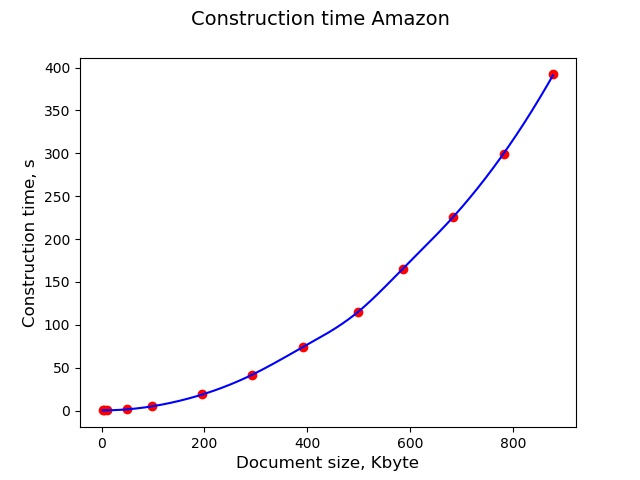
\includegraphics[width=12cm]{construct_time_amazon}
	\caption{Построение CSA}
	\label{fig:CSA_construct_time_amazon}
\end{figure}

\begin{figure}[h!]
	\centering
	\begin{subfigure}[b]{0.49\textwidth}
		\centering
		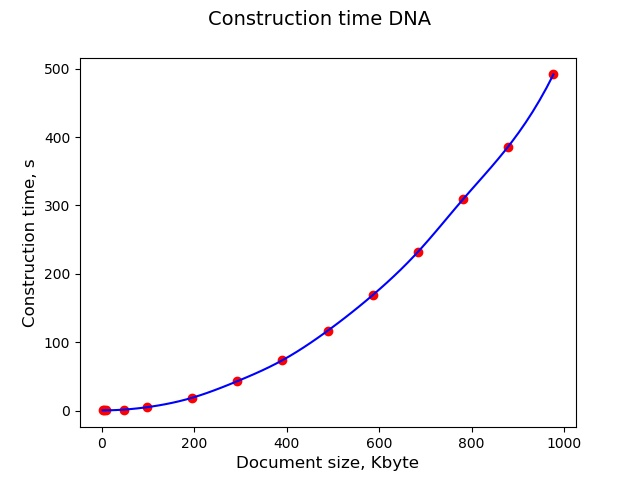
\includegraphics[width=\textwidth]{construct_time_DNA}
		\caption{DNA}
		\label{fig:y equals x}
	\end{subfigure}
	\hfill
	\begin{subfigure}[b]{0.49\textwidth}
		\centering
		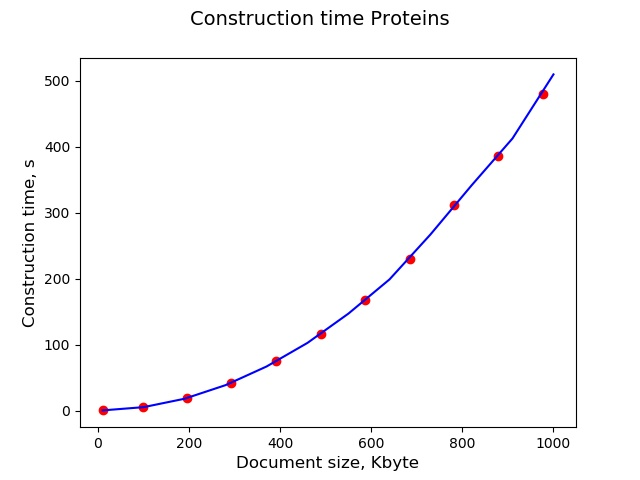
\includegraphics[width=\textwidth]{construct_time_Proteins}
		\caption{Proteins}
		\label{fig:three sin x}
	\end{subfigure}
	\hfill
	\begin{subfigure}[b]{0.49\textwidth}
		\centering
		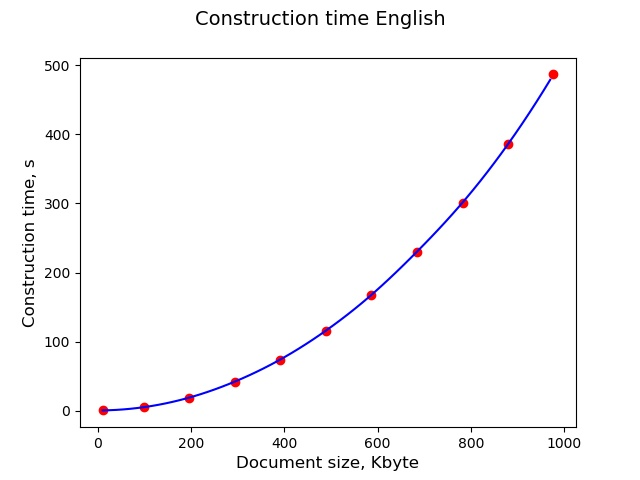
\includegraphics[width=\textwidth]{construct_time_English}
		\caption{English}
		\label{fig:three sin x}
	\end{subfigure}
	\hfill
	\begin{subfigure}[b]{0.49\textwidth}
		\centering
		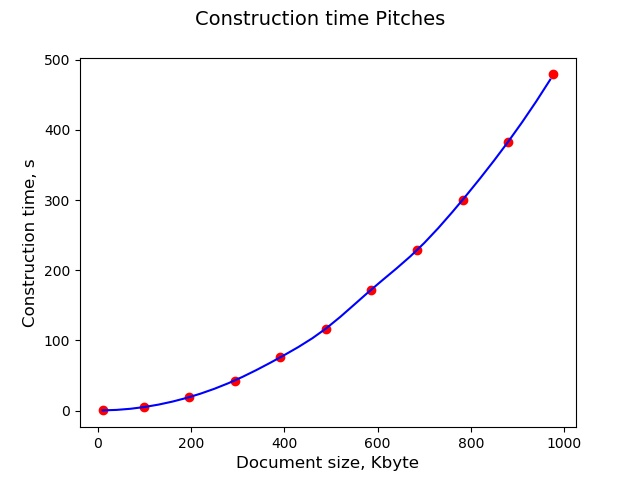
\includegraphics[width=\textwidth]{construct_time_Pitches}
		\caption{Pitches}
		\label{fig:three sin x}
	\end{subfigure}
	\caption{Построение CSA}
	\label{fig:three graphs}
\end{figure}

\begin{figure}[h!]
	\centering
	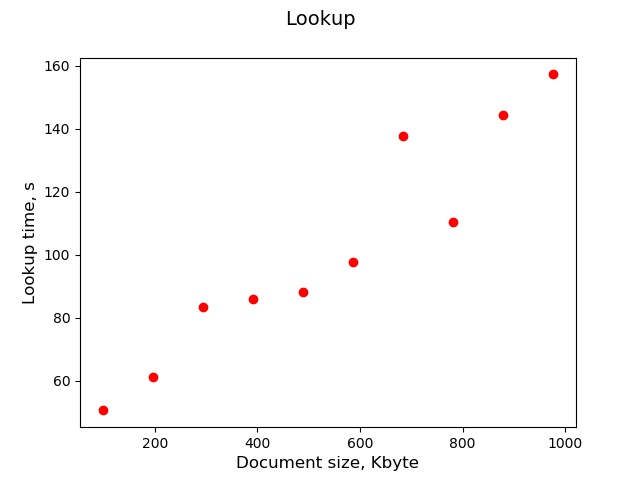
\includegraphics[width=12cm]{Lookup_time_csa_amazon}
	\caption{Поиск подстроки в CSA}
	\label{fig:CSA_Lookup_time_csa_amazon}
\end{figure}

\clearpage
\newpage
Рассмотрим результаты зависимость скорости поиска подстроки от размера текста для CSA,
suffix array и radix tree, построенных для Amazon Text Corpora. На рисунке \ref{fig:CSA_Lookup_time}
можно видеть, что скорость поиска подстроки фиксированного размера не зависит от размера текста
для suffix array и radix tree. Для CSA время поиска увеличивается при увеличении размера исходного текста.
Radix tree, как ожидалось, показывает лучший результат.

\begin{figure}[h!]
	\centering
	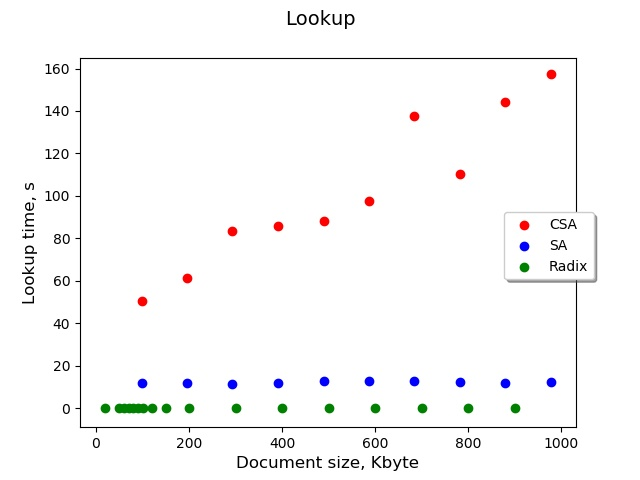
\includegraphics[width=12cm]{Lookup_time}
	\caption{Поиск подстроки в CSA}
	\label{fig:CSA_Lookup_time}
\end{figure}

